\documentclass{article}
\usepackage{tikz}
\usetikzlibrary{mindmap,positioning}

\begin{document}

\section{Izbira modela}
\subsection{Osrednja arhitektura}
\begin{itemize}
    \item{Pristopi so bili ovrednoteni posamično, s predpostavko medsebojne neodvisnosti (zaradi zahtevnosti treniranja)}
    \item{Modeli vrednoteni relativno med vozlišči na istem nivoju grafa}

    \item{Označbe metod:}
    \begin{itemize}
        \item{Siva - nepreizkušeno}
        \item{Zelena - izbrano za končni model}
        \item{Rdeča - neizbrano/slabše}
        \item{Modra - primerjava ni nujno primerna}
        \item{Rumena - ne predstavlja opazne izboljšave}
    \end{itemize}
\end{itemize}

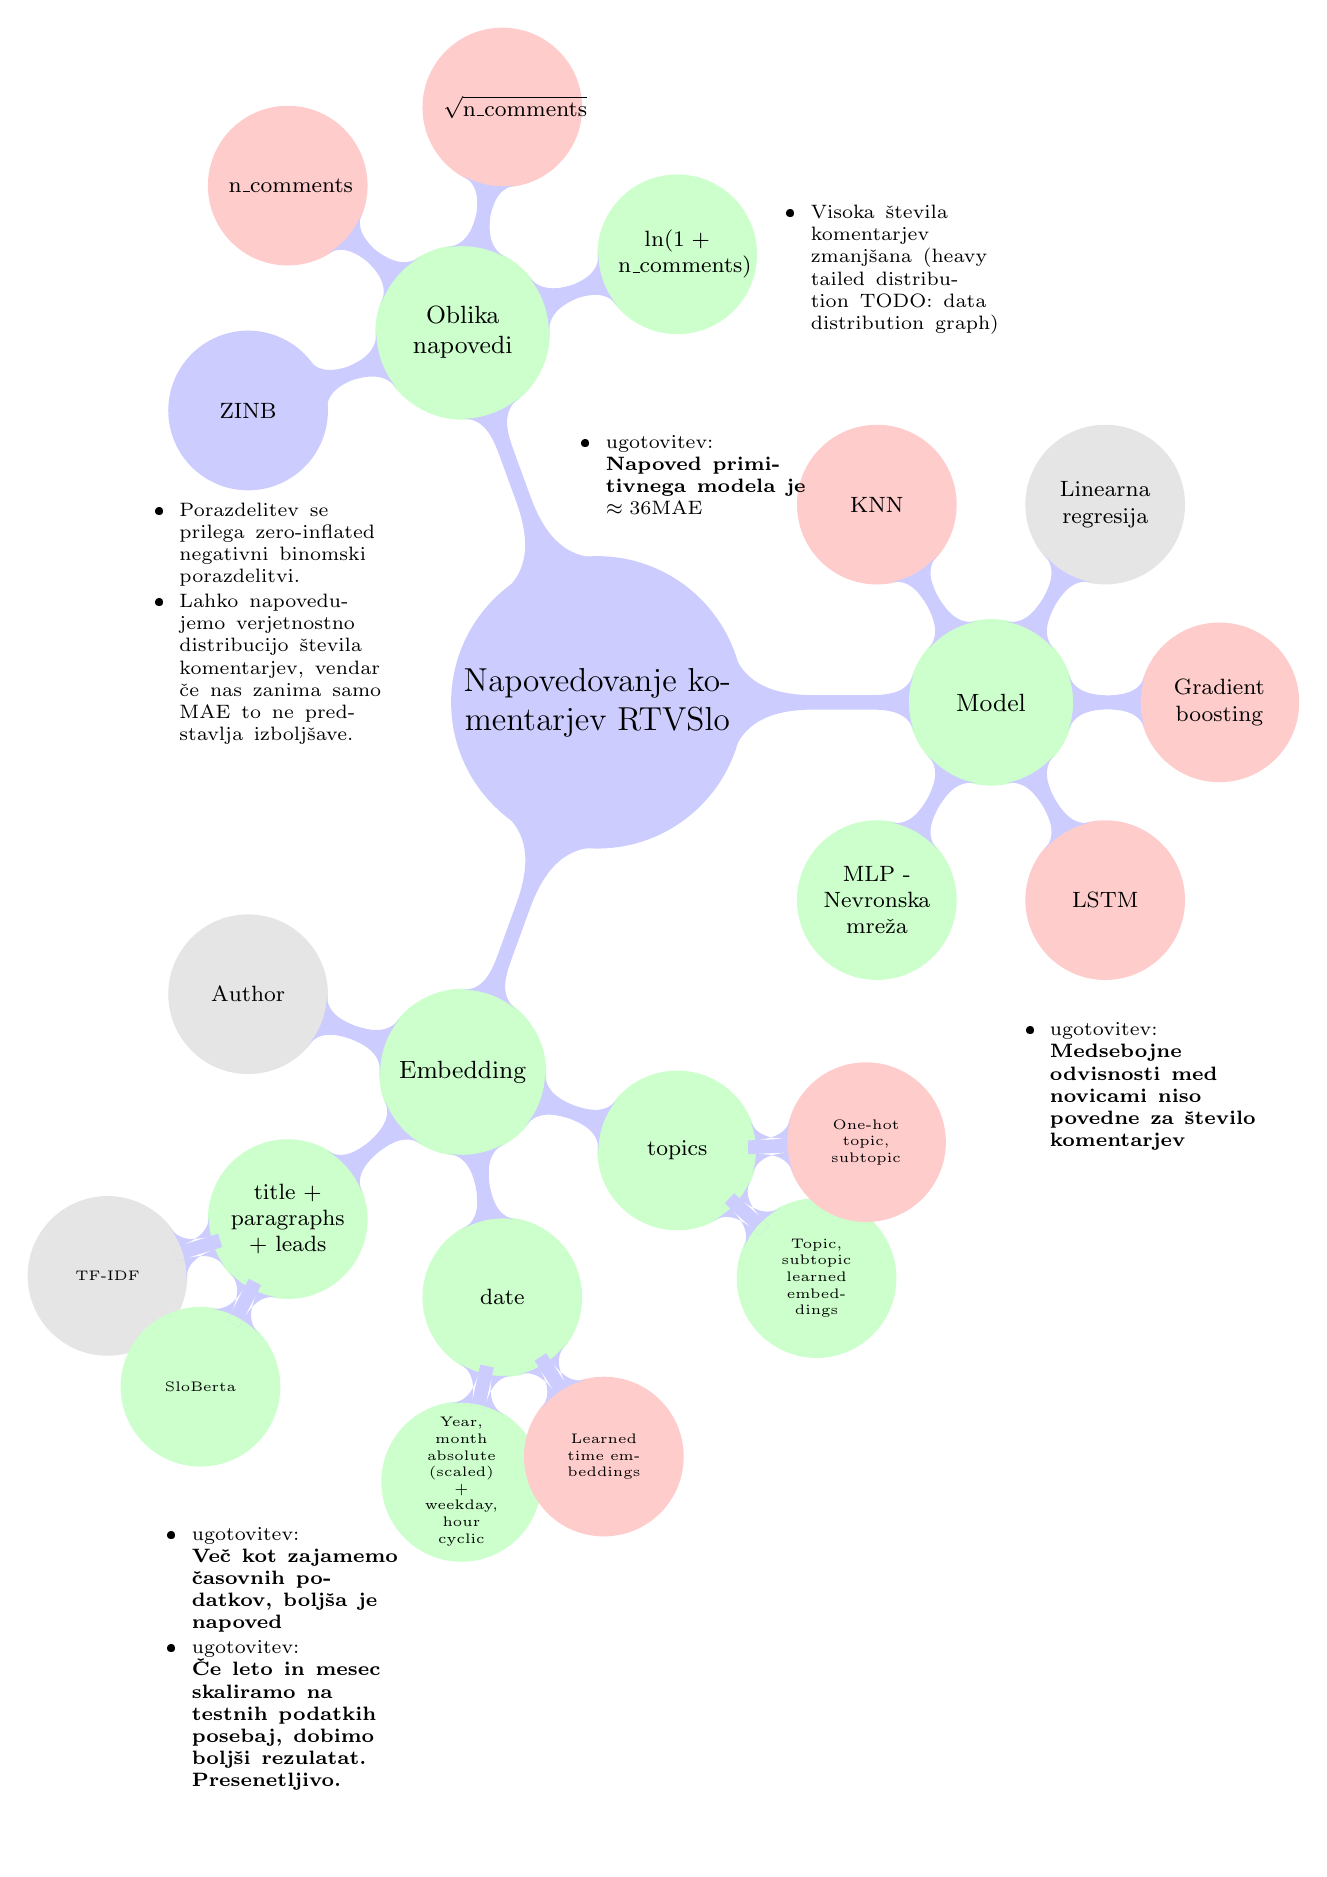
\begin{tikzpicture}[mindmap,
    every node/.style={concept, draw, circle, thick, text=black, minimum size=2cm},
    concept color=blue!20,
    grow cyclic,
    level 1/.append style={sibling angle=110},
    level 2/.append style={sibling angle=60},
    level 3/.append style={sibling angle=45},
    ]
  \node {Napovedovanje komentarjev RTVSlo}
      child { node[concept color=green!20] {Embedding}
          child { node[concept color=gray!20] {Author} }
          child { node[concept color=green!20] {title + paragraphs + leads}
              child { node[concept color=gray!20] {TF-IDF} }
              child { node[concept color=green!20] {SloBerta} }
          }
          child { node[concept color=green!20] {date}
              child { node[concept color=green!20] (datetime) {Year, month absolute (scaled) + weekday, hour cyclic} }
              child { node[concept color=red!20] {Learned time embeddings} }
          }
          child { node[concept color=green!20] {topics}
              child { node[concept color=green!20] {Topic, subtopic learned embeddings} }
              child { node[concept color=red!20] {One-hot topic, subtopic} }
          }
        }
      child { node[concept color=green!20] {Model}
          child { node[concept color=green!20] {MLP - Nevronska mreža} }
          child { node[concept color=red!20] (lstm) {LSTM} }
          child { node[concept color=red!20] {Gradient boosting} }
          child { node[concept color=gray!20] (linreg) {Linearna regresija} }
          child { node[concept color=red!20] (knn) {KNN} }
        }
      child { node[concept color=green!20] {Oblika napovedi}
          child { node[concept color=green!20] (log) {$\ln(1 + \mathrm{n\_comments})$} }
          child { node[concept color=red!20] {$\sqrt{\mathrm{n\_comments}}$} }
          child { node[concept color=red!20] {n\_comments} }
          child { node[concept color=blue!20] (zinb) {ZINB} }
        };

\node[draw=none, fill=none, text=black, below left=-5mm and 0mm of datetime] {
  \scriptsize
  \begin{itemize}
    \setlength\itemsep{1pt}        % spacing between items
    \setlength\parskip{0pt}        % paragraph spacing
    \setlength\parsep{0pt}         % spacing between item and paragraph
    \item ugotovitev: \\ \textbf{Več kot zajamemo časovnih podatkov, boljša je napoved}
    \item ugotovitev: \\ \textbf{Če leto in mesec skaliramo na testnih podatkih posebaj, dobimo boljši rezulatat. Presenetljivo.}
  \end{itemize}
};

\node[draw=none, fill=none, text=black, below right=0mm and -20mm of lstm] {
  \scriptsize
  \begin{itemize}
    \setlength\itemsep{1pt}        % spacing between items
    \setlength\parskip{0pt}        % paragraph spacing
    \setlength\parsep{0pt}         % spacing between item and paragraph
    \item ugotovitev: \\ \textbf{Medsebojne odvisnosti med novicami niso povedne za število komentarjev}
  \end{itemize}
};

\node[draw=none, fill=none, text=black, above left=-15mm and 5mm of knn] {
  \scriptsize
  \begin{itemize}
    \setlength\itemsep{1pt}        % spacing between items
    \setlength\parskip{0pt}        % paragraph spacing
    \setlength\parsep{0pt}         % spacing between item and paragraph
    \item ugotovitev: \\ \textbf{Napoved primitivnega modela je $\approx 36\mathrm{MAE}$}
  \end{itemize}
};

\node[draw=none, fill=none, text=black, right=-5mm of log] {
  \scriptsize
  \begin{itemize}
    \setlength\itemsep{1pt}        % spacing between items
    \setlength\parskip{0pt}        % paragraph spacing
    \setlength\parsep{0pt}         % spacing between item and paragraph
    \item Visoka števila komentarjev zmanjšana (heavy tailed distribution TODO: data distribution graph)
  \end{itemize}
};

\node[draw=none, fill=none, text=black, below=-10mm of zinb] {
  \scriptsize
  \begin{itemize}
    \setlength\itemsep{1pt}        % spacing between items
    \setlength\parskip{0pt}        % paragraph spacing
    \setlength\parsep{0pt}         % spacing between item and paragraph
    \item Porazdelitev se prilega zero-inflated negativni binomski porazdelitvi.
    \item Lahko napovedujemo verjetnostno distribucijo števila komentarjev, vendar če nas zanima samo MAE to ne predstavlja izboljšave.
  \end{itemize}
};

\end{tikzpicture}

\subsection{Nadgradnje in ostale analize}
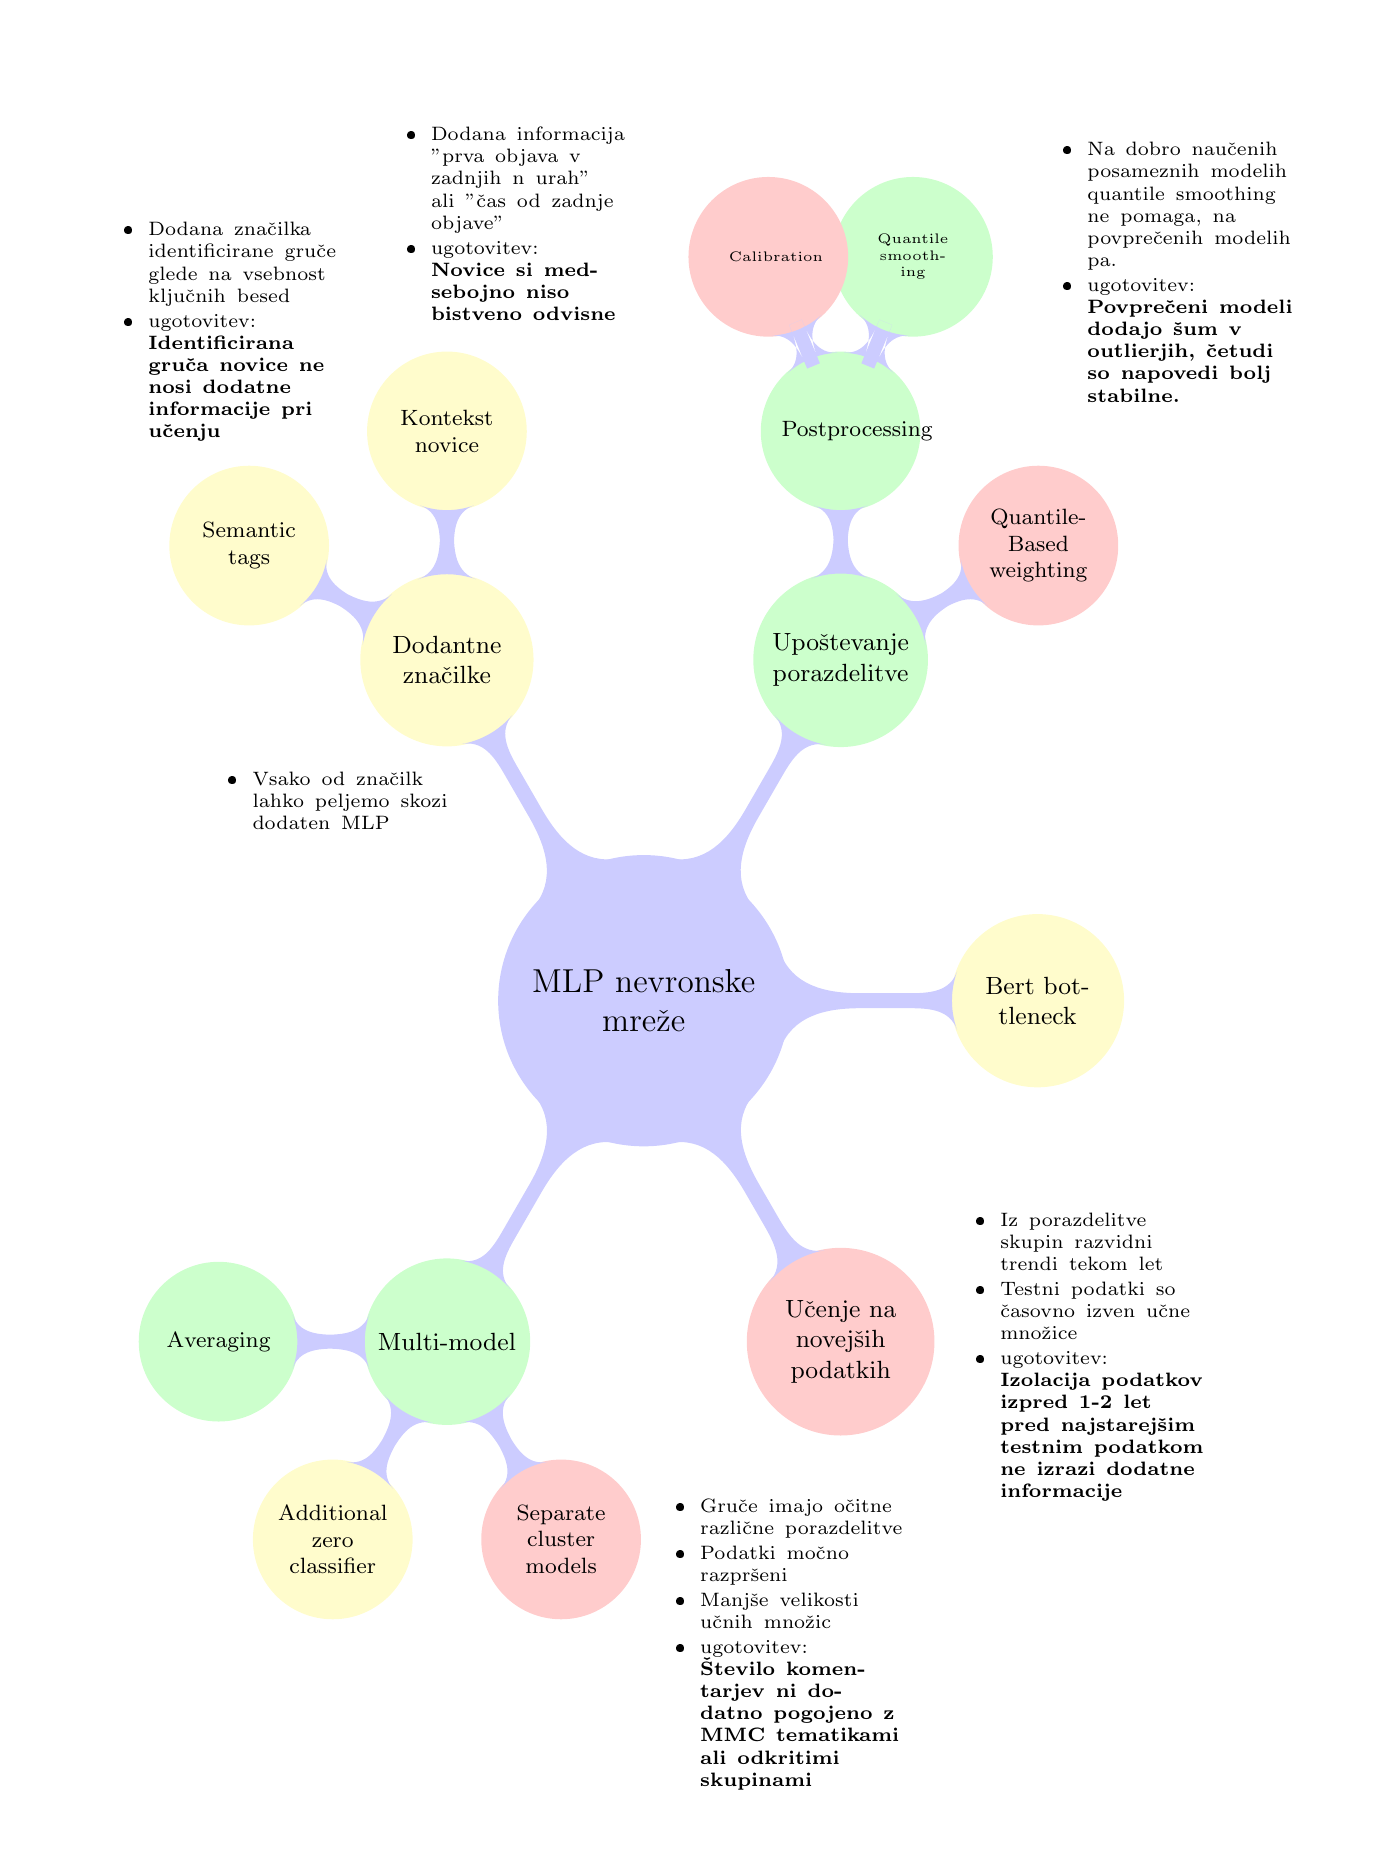
\begin{tikzpicture}[mindmap,
    every node/.style={concept, draw, circle, thick, text=black, minimum size=2cm},
    concept color=blue!20,
    grow cyclic,
    level 1/.append style={sibling angle=60},
    level 2/.append style={sibling angle=60},
    level 3/.append style={sibling angle=45},
    ]
  \node {MLP nevronske mreže}
      child { node[concept color=green!20] {Multi-model}
          child { node[concept color=green!20] {Averaging} }
          child { node[concept color=yellow!20] {Additional zero classifier} }
          child { node[concept color=red!20] (clusters) {Separate cluster models} }
        }
      child { node[concept color=red!20] (yearcutoff) {Učenje na novejših podatkih} }
      child { node[concept color=yellow!20] (bottleneck) {Bert bottleneck} }
      child { node[concept color=green!20] {Upoštevanje porazdelitve} 
          child { node[concept color=red!20] {Quantile-Based weighting} }
          child { node[concept color=green!20] {Postprocessing} 
              child { node[concept color=green!20] (quantilesmoothing) {Quantile smoothing} }
              child { node[concept color=red!20] (calibration) {Calibration}}
          }
        }
      child { node[concept color=yellow!20] (additionalfeats) {Dodantne značilke} 
          child { node[concept color=yellow!20] (context) {Kontekst novice} }
          child { node[concept color=yellow!20] (semantic) {Semantic tags} }
        };

\node[draw=none, fill=none, text=black, below right=-15mm and 0mm of clusters] {
  \scriptsize
  \begin{itemize}
    \setlength\itemsep{1pt}        % spacing between items
    \setlength\parskip{0pt}        % paragraph spacing
    \setlength\parsep{0pt}         % spacing between item and paragraph
    \item Gruče imajo očitne različne porazdelitve
    \item Podatki močno razpršeni
    \item Manjše velikosti učnih množic
    \item ugotovitev: \\ \textbf{Število komentarjev ni dodatno pogojeno z MMC tematikami ali odkritimi skupinami}
  \end{itemize}
};

\node[draw=none, fill=none, text=black, right=-10mm of yearcutoff] {
  \scriptsize
  \begin{itemize}
    \setlength\itemsep{1pt}        % spacing between items
    \setlength\parskip{0pt}        % paragraph spacing
    \setlength\parsep{0pt}         % spacing between item and paragraph
    \item Iz porazdelitve skupin razvidni trendi tekom let
    \item Testni podatki so časovno izven učne množice
    \item ugotovitev: \\ \textbf{Izolacija podatkov izpred 1-2 let pred najstarejšim testnim podatkom ne izrazi dodatne informacije}
  \end{itemize}
};

\node[draw=none, fill=none, text=black, right=-5mm of quantilesmoothing] {
  \scriptsize
  \begin{itemize}
    \setlength\itemsep{1pt}        % spacing between items
    \setlength\parskip{0pt}        % paragraph spacing
    \setlength\parsep{0pt}         % spacing between item and paragraph
    \item Na dobro naučenih posameznih modelih quantile smoothing ne pomaga, na povprečenih modelih pa.
    \item ugotovitev: \\ \textbf{Povprečeni modeli dodajo šum v outlierjih, četudi so napovedi bolj stabilne.}
  \end{itemize}
};

\node[draw=none, fill=none, text=black, below left=-5mm and -5mm of additionalfeats] {
  \scriptsize
  \begin{itemize}
    \setlength\itemsep{1pt}        % spacing between items
    \setlength\parskip{0pt}        % paragraph spacing
    \setlength\parsep{0pt}         % spacing between item and paragraph
    \item Vsako od značilk lahko peljemo skozi dodaten MLP
  \end{itemize}
};

\node[draw=none, fill=none, text=black, above left=5mm and -30mm of context] {
  \scriptsize
  \begin{itemize}
    \setlength\itemsep{1pt}        % spacing between items
    \setlength\parskip{0pt}        % paragraph spacing
    \setlength\parsep{0pt}         % spacing between item and paragraph
    \item Dodana informacija "prva objava v zadnjih n urah" ali "čas od zadnje objave"
    \item ugotovitev: \\ \textbf{Novice si medsebojno niso bistveno odvisne}
  \end{itemize}
};

\node[draw=none, fill=none, text=black, above left=5mm and -20mm of semantic] {
  \scriptsize
  \begin{itemize}
    \setlength\itemsep{1pt}        % spacing between items
    \setlength\parskip{0pt}        % paragraph spacing
    \setlength\parsep{0pt}         % spacing between item and paragraph
    \item Dodana značilka identificirane gruče glede na vsebnost ključnih besed
    \item ugotovitev: \\ \textbf{Identificirana gruča novice ne nosi dodatne informacije pri učenju}
  \end{itemize}
};


\end{tikzpicture}

\section{Vrednotenje}
\section{Razlaga}


\end{document}

